\section{Results}\label{sec:results}
We estimate the effects (coefficients of the model) by minimizing the the residue in the sense of least square as expressed by eq. \ref{eq:least_square}.
\begin{equation}\label{eq:least_square}
	\hat\alpha =  \argmin_{\alpha}{(\sum_{k = 1}^{N} (y_{ak} -  X_{k}\alpha)^2)}
\end{equation}
$\hat\alpha$ are the estimated half effects, $N$ the number of experiments, $y_{ak}$ is the result of the $k$th experiment for response $a$ and $X_k$ is the $k$th row of the model matrix $X$ containing the values for each parameter as well as the corresponding effects and $\alpha$ are the half effects.
We define the dispersion matrix $D$ of the model as
\begin{equation}
	D = (X^T X)^{-1}.
\end{equation}
The solution to eq. \ref{eq:least_square} can be computed as
\begin{equation}
	\hat\alpha = D X^{T} Y.
\end{equation}

%The results of the simulation versus the parameter values are shown in fig. \ref{fig:results_y}.

%\begin{figure}
%    \centering
%    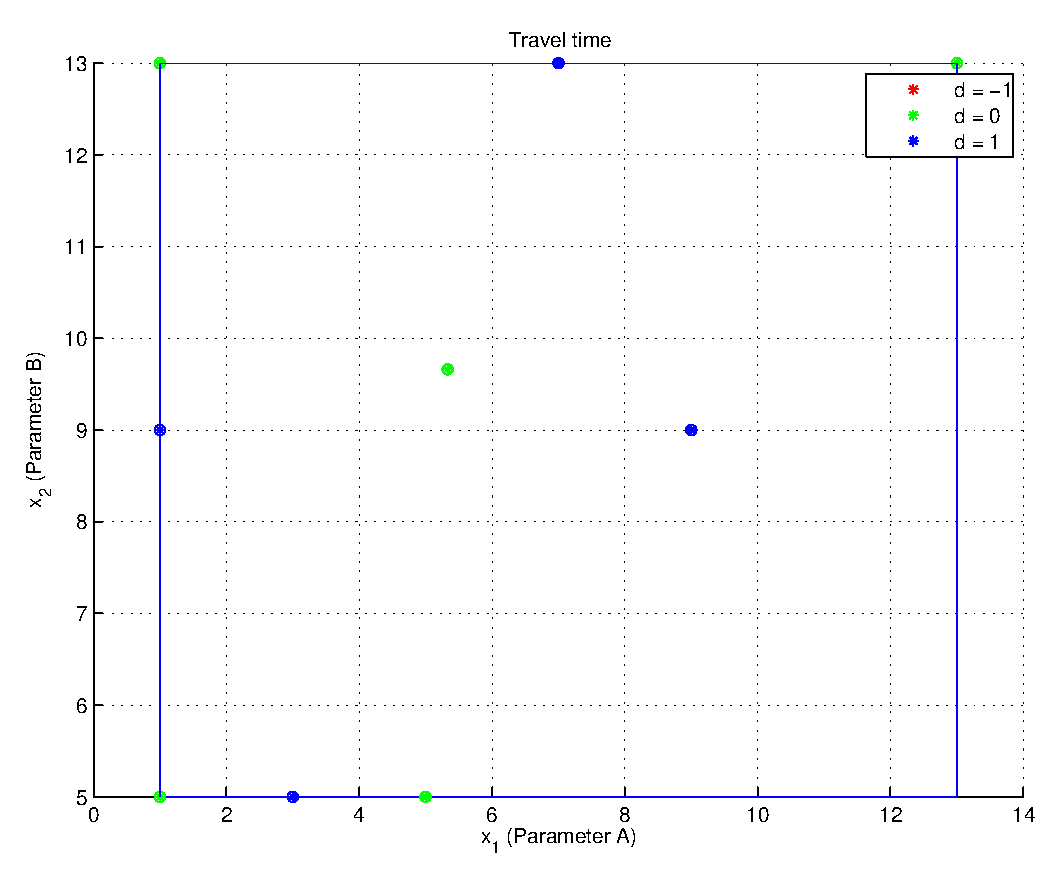
\includegraphics{images/epsFig}
%    \caption{Insert caption}
%\end{figure} 
\subsection{Linear Model}
First, we will discuss the results for the linear model.
Fig. \ref{fig:effects_lin} shows the half effects for both the travel time and the jerk in blue. It can be seen that the influence of parameter A (coefficients $a_1$ and $b_1$) on both the travel time and the jerk is negligible compared to the other effects.
\begin{figure}[h]
    \centering
    \begin{subfigure}[b]{0.5\textwidth}
		\setlength{\abovecaptionskip}{1pt plus 3pt minus 0pt}	
	    % This file was created by matlab2tikz.
%
\definecolor{mycolor1}{rgb}{0.20000,0.20000,0.50000}%
\definecolor{mycolor2}{rgb}{0.00000,0.70000,0.70000}%
%
\begin{tikzpicture}

\begin{axis}[%
width=0.951\figW,
height=\figH,
at={(0\figW,0\figH)},
scale only axis,
separate axis lines,
every outer x axis line/.append style={black},
every x tick label/.append style={font=\color{black}},
xmin=0.5,
xmax=4.5,
xtick={1,2,3,4},
xticklabels={{$a_0$},{$a_1$},{$a_2$},{$a_3$},{$a_{12}$},{$a_{13}$},{$a_{23}$},{$a_{11}$},{$a_{22}$},{$a_{33}$}},
xlabel={coefficients},
every outer y axis line/.append style={black},
every y tick label/.append style={font=\color{black}},
ymin=0,
ymax=1,
ylabel={$\text{a}_\text{i}\text{/a}_\text{0}$},
axis background/.style={fill=white},
xlabel shift={-4pt},
ylabel shift={-4pt}
]
\addplot[ybar,bar width=0.5,draw=black,fill=mycolor1,area legend] plot table[row sep=crcr] {%
1	1\\
2	0.00339552585792994\\
3	0.27192029312426\\
4	0.201983314513812\\
};
\addplot [color=black,solid,forget plot]
  table[row sep=crcr]{%
0.5	0\\
4.5	0\\
};
\addplot[ybar,bar width=0.25,draw=black,fill=mycolor2,area legend] plot table[row sep=crcr] {%
1	0.998868158047356\\
3	0.273052135076903\\
4	0.201983314513812\\
};
\end{axis}
\end{tikzpicture}%
	    \caption{travel time}
	\end{subfigure}
	%\par\medskip
    \begin{subfigure}[b]{0.5\textwidth}
	    \setlength{\abovecaptionskip}{1pt plus 3pt minus 0pt}
	    % This file was created by matlab2tikz.
%
\definecolor{mycolor1}{rgb}{0.20000,0.20000,0.50000}%
\definecolor{mycolor2}{rgb}{0.00000,0.70000,0.70000}%
%
\begin{tikzpicture}

\begin{axis}[%
width=0.951\figW,
height=\figH,
at={(0\figW,0\figH)},
scale only axis,
separate axis lines,
every outer x axis line/.append style={black},
every x tick label/.append style={font=\color{black}},
xmin=0.5,
xmax=4.5,
xtick={1,2,3,4},
xticklabels={{$b_0$},{$b_1$},{$b_2$},{$b_3$},{$b_{12}$},{$b_{13}$},{$b_{23}$},{$b_{11}$},{$b_{22}$},{$b_{33}$}},
xlabel={coefficients},
every outer y axis line/.append style={black},
every y tick label/.append style={font=\color{black}},
ymin=0,
ymax=1,
ylabel={bi/bo},
axis background/.style={fill=white},
xlabel shift={-4pt},
ylabel shift={-5pt}
]
\addplot[ybar,bar width=0.5,draw=black,fill=mycolor1,area legend] plot table[row sep=crcr] {%
1	1\\
2	0.0572355129983193\\
3	0.822964208269701\\
4	0.479348852445352\\
};
\addplot [color=black,solid,forget plot]
  table[row sep=crcr]{%
0.5	0\\
4.5	0\\
};
\addplot[ybar,bar width=0.25,draw=black,fill=mycolor2,area legend] plot table[row sep=crcr] {%
1	0.980921495667227\\
3	0.842042712602474\\
4	0.479348852445352\\
};
\end{axis}
\end{tikzpicture}%
   	    \caption{jerk}
	\end{subfigure}
	
    \caption{Relative half effects on the mean travel time (a) and the mean experienced jerk (b) using a linear model without interactions; In blue results for using all parameters and in turquoise if omitting parameter A (coefficients $a1$ and $b1$)}\label{fig:effects_lin}
\end{figure} 

The ANOVA table is shown in tbl. \ref{tbl:anova_lin_time} for the mean travel time and in tbl. \ref{tbl:anova_lin_jerk} for the mean experienced jerk. The p-value for the travel time model (2.35e-7) is significantly lower than the p-value for jerk model (4.72e-2). This suggest that the travel time model fits much better the experimental data.

\begin{table}[h!]
	\centering
	\begin{tabular}{l r r r r r}
	%\thickline
	    Source	 & SS      	 & df      	 & MS      	 & F       	 & p        \\\hline
  Constant	 & 34.4  	 & 4     	 & 8.61  	 & 95    	 & 2.35e-07\\
   Residue	 & 0.815 	 & 9     	 & 0.0906 

	\end{tabular}
	
	\bigskip

	\begin{tabular}{l r r r r r}
	%\thickline
	    Source	 & SS      	 & df      	 & MS      	 & F       	 & p        \\\hline
  Constant	 & 34.4  	 & 3     	 & 11.5  	 & 141   	 & 1.78e-08\\
   Residue	 & 0.815 	 & 10    	 & 0.0815 
	
	\end{tabular}
	\caption{ANOVA table of the \textbf{linear model} for the mean \textbf{travel time}; Top: full linear model; Bottom: omitting parameter A (coefficient $a1$); It shows the sums of squares (SS), the degrees of freedom (df), the mean square of the error (MS), the Fisher coefficient (F) and the p-value (p), signifying the probability that this result occurs at random;}\label{tbl:anova_lin_time}
\end{table}

Fig. \ref{fig:interpol_lin1} shows the experimental results for the travel time as well as the planes representing the interpolation using the effects that we have found. The colors correspond to different values of parameter C, i.e., the dots should be close to the plane of the same color. Fig. \ref{fig:interpol_lin2} shows the results in terms of jerk. Note that here the colors correspond to the value of the parameter A. It can be seen that the points for measurements with the same values for parameter B and C are close by, encouraging the assumption that the influence of parameter A is negligible.

We therefore adjust both our models by omitting parameter A. We expect the residue to increase slightly since we remove a degree of freedom. The removal of a degree of freedom should however increase F-factor and therefore reduce the p-value, since the residue gains a degree of freedom. The resulting estimation of the half effects is shown in fig. \ref{fig:effects_lin} in turquoise. It can be seen that the values of the half effects are similar to the previous results.

 When comparing the ANOVA tables for the travel time (tbl. \ref{tbl:anova_lin_time}), it can be seen that the $p$ value decreases by a factor of approximately 13, suggesting that omitting parameter A is improving our model. For the model of the jerk, the p-value   decreases by a factor of approximately 2.7 (cf. tbl. \ref{tbl:anova_lin_jerk}).
\begin{figure}
    \centering
    \setlength{\abovecaptionskip}{1pt plus 3pt minus 0pt}
	% This file was created by matlab2tikz.
%
%The latest updates can be retrieved from
%  http://www.mathworks.com/matlabcentral/fileexchange/22022-matlab2tikz-matlab2tikz
%where you can also make suggestions and rate matlab2tikz.
%
\begin{tikzpicture}

\begin{axis}[%
width=0.951\figW,
height=\figH,
at={(0\figW,0\figH)},
scale only axis,
every outer x axis line/.append style={black},
every x tick label/.append style={font=\color{black}},
xmin=0,
xmax=14,
xlabel={$\text{x}_\text{1}\text{ (Parameter A)}$},
xmajorgrids,
every outer y axis line/.append style={black},
every y tick label/.append style={font=\color{black}},
ymin=5,
ymax=13,
ylabel={$\text{x}_\text{2}\text{ (Parameter B)}$},
ymajorgrids,
axis background/.style={fill=white},
title={Travel time},
axis x line*=bottom,
axis y line*=left,
legend style={legend cell align=left,align=left,draw=black}
]
\addplot [color=red,mark size=2.5pt,only marks,mark=asterisk,mark options={solid}]
  table[row sep=crcr]{%
1	9\\
9	9\\
3	5\\
7	13\\
};
\addlegendentry{d = -1};

\addplot [color=green,mark size=2.5pt,only marks,mark=asterisk,mark options={solid}]
  table[row sep=crcr]{%
1	5\\
1	13\\
5	5\\
13	13\\
5.33	9.66\\
};
\addlegendentry{d = 0};

\addplot [color=blue,mark size=2.5pt,only marks,mark=asterisk,mark options={solid}]
  table[row sep=crcr]{%
1	9\\
9	9\\
3	5\\
7	13\\
};
\addlegendentry{d = 1};

\addplot [color=red,mark size=2.5pt,only marks,mark=o,mark options={solid},forget plot]
  table[row sep=crcr]{%
1	9\\
9	9\\
3	5\\
7	13\\
};
\addplot [color=green,mark size=2.5pt,only marks,mark=o,mark options={solid},forget plot]
  table[row sep=crcr]{%
1	5\\
1	13\\
5	5\\
13	13\\
5.33	9.66\\
};
\addplot [color=blue,mark size=2.5pt,only marks,mark=o,mark options={solid},forget plot]
  table[row sep=crcr]{%
1	9\\
9	9\\
3	5\\
7	13\\
};
\addplot [color=blue,solid,forget plot]
  table[row sep=crcr]{%
1	5\\
1	13\\
13	13\\
13	5\\
1	5\\
};
\end{axis}
\end{tikzpicture}%
    \caption{Insert caption}
\end{figure}


\begin{table}[h!]
	\centering

	\begin{tabular}{l r r r r r}
	%\thickline
	    Source	 & SS      	 & df      	 & MS      	 & F       	 & p        \\\hline
  Constant	 & 2.41e+03	 & 4     	 & 601   	 & 3.72  	 & 0.0472\\
   Residue	 & 1.46e+03	 & 9     	 & 162    

	\end{tabular}

	\bigskip

	\begin{tabular}{l r r r r r}
	%\thickline	
	    Source	 & SS      	 & df      	 & MS      	 & F       	 & p        \\\hline
  Constant	 & 2.4e+03	 & 3     	 & 801   	 & 5.5   	 & 0.0172\\
   Residue	 & 1.46e+03	 & 10    	 & 146    
	
	\end{tabular}

	\caption{ANOVA table of the \textbf{linear model} for the mean experienced \textbf{jerk}; Top: full linear model; Bottom: omitting parameter A (coefficient $b1$)}\label{tbl:anova_lin_jerk}
\end{table}


\subsection{Linear Model with interactions}

\begin{figure}[h]
    \centering
    \begin{subfigure}[b]{0.5\textwidth}
	    \setlength{\abovecaptionskip}{1pt plus 3pt minus 0pt}
	    % This file was created by matlab2tikz.
%
\definecolor{mycolor1}{rgb}{0.20000,0.20000,0.50000}%
\definecolor{mycolor2}{rgb}{0.00000,0.70000,0.70000}%
%
\begin{tikzpicture}

\begin{axis}[%
width=0.951\figW,
height=\figH,
at={(0\figW,0\figH)},
scale only axis,
separate axis lines,
every outer x axis line/.append style={black},
every x tick label/.append style={font=\color{black}},
xmin=0,
xmax=8,
xtick={1,2,3,4,5,6,7},
xticklabels={{$a_0$},{$a_1$},{$a_2$},{$a_3$},{$a_{12}$},{$a_{13}$},{$a_{23}$},{$a_{11}$},{$a_{22}$},{$a_{33}$}},
xlabel={coefficients},
every outer y axis line/.append style={black},
every y tick label/.append style={font=\color{black}},
ymin=-0.2,
ymax=1.2,
ylabel={ai/ao},
axis background/.style={fill=white},
xlabel shift={-4pt}
]
\addplot[ybar,bar width=0.5,draw=black,fill=mycolor1,area legend] plot table[row sep=crcr] {%
1	1\\
2	-0.000158480987423072\\
3	0.276585231712786\\
4	0.202308189537893\\
5	0.00801820250102874\\
6	-0.000745454946096567\\
7	0.116456628245764\\
};
\addplot [color=black,solid,forget plot]
  table[row sep=crcr]{%
0	0\\
8	0\\
};
\addplot[ybar,bar width=0.25,draw=black,fill=mycolor2,area legend] plot table[row sep=crcr] {%
1	1\\
3	0.273361537132869\\
4	0.202212186750112\\
7	0.116010508284771\\
};
\end{axis}
\end{tikzpicture}%
	    \caption{travel time}
	\end{subfigure}
    \begin{subfigure}[b]{0.5\textwidth}
		\setlength{\abovecaptionskip}{1pt plus 3pt minus 0pt}	
	    % This file was created by matlab2tikz.
%
\definecolor{mycolor1}{rgb}{0.20000,0.20000,0.50000}%
\definecolor{mycolor2}{rgb}{0.00000,0.70000,0.70000}%
%
\begin{tikzpicture}

\begin{axis}[%
width=0.951\figW,
height=\figH,
at={(0\figW,0\figH)},
scale only axis,
separate axis lines,
every outer x axis line/.append style={black},
every x tick label/.append style={font=\color{black}},
xmin=0,
xmax=8,
xtick={1,2,3,4,5,6,7},
xticklabels={{$b_0$},{$b_1$},{$b_2$},{$b_3$},{$b_{12}$},{$b_{13}$},{$b_{23}$},{$b_{11}$},{$b_{22}$},{$b_{33}$}},
xlabel={coefficients},
every outer y axis line/.append style={black},
every y tick label/.append style={font=\color{black}},
ymin=-0.2,
ymax=1.2,
ylabel={bi/bo},
axis background/.style={fill=white},
xlabel shift={-4pt}
]
\addplot[ybar,bar width=0.5,draw=black,fill=mycolor1,area legend] plot table[row sep=crcr] {%
1	1\\
2	0.0492031949956049\\
3	0.837675184978511\\
4	0.479930485262015\\
5	0.0189360359982001\\
6	-0.0078955424930121\\
7	0.0133129711999519\\
};
\addplot [color=black,solid,forget plot]
  table[row sep=crcr]{%
0	0\\
8	0\\
};
\addplot[ybar,bar width=0.25,draw=black,fill=mycolor2,area legend] plot table[row sep=crcr] {%
1	1\\
3	0.858420083892354\\
4	0.488671982990134\\
};
\end{axis}
\end{tikzpicture}%
   	    \caption{jerk}
	\end{subfigure}
	
    \caption{Relative half effects on the mean travel time (a) and the mean experienced jerk (b) using a \textbf{linear model with interactions}; In blue results for using all parameters and in turquoise if omitting coefficients $a1$, $a12$ and $a13$ and $b1$, $b12$, $b13$, and $b23$)}\label{fig:effects_lin_interactions}
\end{figure} 
Fig. \ref{fig:effects_lin_interactions} shows the effects for this model. For both response variables we can again see that the influences of parameter A is negligible as it was the case for the purely linear model. Furthermore, the interactions appear to be negligible in the case of the jerk model. Considering the ANOVA table for this model (tbl. \ref{tbl:anova_lin_interactions_time} and tbl. \ref{tbl:anova_lin_interactions_jerk}), it can be seen that the p value is significantly higher than for the linear model. This suggests that the addition of the interactions does not improve the model. This is due to the fact that the number of degrees of freedom of the models increase significantly were as whereas the residues remain approximately the same as for the linear models. While removing parameter A from the travel time model reduces it's p-value, it still remains inferior to the linear model.

\begin{table}[h!]
	\centering

	\begin{tabular}{l r r r r r}
	%\thickline
	    Source	 & SS      	 & df      	 & MS      	 & F       	 & p        \\\hline
  Constant	 & 34.6  	 & 7     	 & 4.94  	 & 43.4  	 & 0.000101\\
   Residue	 & 0.682 	 & 6     	 & 0.114  

	\end{tabular}

	\bigskip

	\begin{tabular}{l r r r r r}
	%\thickline	
	    Source	 & SS      	 & df      	 & MS      	 & F       	 & p        \\\hline
  Constant	 & 33.6  	 & 4     	 & 8.4   	 & 46.8  	 & 5.04e-06\\
   Residue	 & 1.62  	 & 9     	 & 0.18   
	
	\end{tabular}

	\caption{ANOVA table of the \textbf{linear model with interactions} for the mean \textbf{travel time}; Top: full linear model with interactions; Bottom: omitting parameter A (coefficients $a1$, $a12$ and $a13$)}\label{tbl:anova_lin_interactions_time}
\end{table}

\begin{table}[h!]
	\centering

	\begin{tabular}{l r r r r r}
	%\thickline
	    Source	 & SS      	 & df      	 & MS      	 & F       	 & p        \\\hline
  Constant	 & 2.41e+03	 & 7     	 & 344   	 & 1.42  	 & 0.344 \\
   Residue	 & 1.46e+03	 & 6     	 & 243    

	\end{tabular}

	%\bigskip

	%\begin{tabular}{l r r r r r}
	%\thickline	
	%    Source	 & SS      	 & df      	 & MS      	 & F       	 & p        \\\hline
  Constant	 & 2.41e+03	 & 7     	 & 344   	 & 1.42  	 & 0.344 \\
   Residue	 & 1.46e+03	 & 6     	 & 243    
	
	%\end{tabular}

	\caption{ANOVA table of the \textbf{linear model with interactions} for the mean experienced \textbf{jerk}}\label{tbl:anova_lin_interactions_jerk}
\end{table}



\subsection{Quadratic Model}

\begin{figure}[h]
    \centering
    \begin{subfigure}[b]{0.5\textwidth}
	    \setlength{\abovecaptionskip}{1pt plus 3pt minus 0pt}
	    % This file was created by matlab2tikz.
%
\definecolor{mycolor1}{rgb}{0.20000,0.20000,0.50000}%
\definecolor{mycolor2}{rgb}{0.00000,0.70000,0.70000}%
%
\begin{tikzpicture}

\begin{axis}[%
width=0.951\figW,
height=\figH,
at={(0\figW,0\figH)},
scale only axis,
separate axis lines,
every outer x axis line/.append style={black},
every x tick label/.append style={font=\color{black}},
xmin=0,
xmax=12,
xtick={1,2,3,4,5,6,7,8,9,10},
xticklabels={{$a_0$},{$a_1$},{$a_2$},{$a_3$},{$a_{12}$},{$a_{13}$},{$a_{23}$},{$a_{11}$},{$a_{22}$},{$a_{33}$}},
xlabel={coefficients},
every outer y axis line/.append style={black},
every y tick label/.append style={font=\color{black}},
ymin=-0.4,
ymax=1,
ylabel={$\text{a}_\text{i}\text{/a}_\text{0}$},
axis background/.style={fill=white},
xlabel shift={-4pt},
ylabel shift={-4pt}
]
\addplot[ybar,bar width=0.5,draw=black,fill=mycolor1,area legend] plot table[row sep=crcr] {%
1	1\\
2	0.239284478024578\\
3	0.120506889726704\\
4	0.204107368761907\\
5	-0.231907710805712\\
6	-0.000752084470361102\\
7	0.117492307258645\\
8	0.358503129231724\\
9	0.0384436095354865\\
10	-0.0964862476571698\\
};
\addplot [color=black,solid,forget plot]
  table[row sep=crcr]{%
0	0\\
12	0\\
};
\addplot[ybar,bar width=0.25,draw=black,fill=mycolor2,area legend] plot table[row sep=crcr] {%
1	1\\
2	0.239284478024579\\
3	0.120506889726704\\
4	0.204358063585361\\
5	-0.231907710805709\\
7	0.117241612435192\\
8	0.358503129231725\\
9	0.0384436095354871\\
10	-0.0964862476571693\\
};
\end{axis}
\end{tikzpicture}%
	    \caption{travel time}
	\end{subfigure}
    \begin{subfigure}[b]{0.5\textwidth}
		\setlength{\abovecaptionskip}{1pt plus 3pt minus 0pt}	
	    % This file was created by matlab2tikz.
%
\definecolor{mycolor1}{rgb}{0.20000,0.20000,0.50000}%
\definecolor{mycolor2}{rgb}{0.00000,0.70000,0.70000}%
%
\begin{tikzpicture}

\begin{axis}[%
width=0.951\figW,
height=\figH,
at={(0\figW,0\figH)},
scale only axis,
separate axis lines,
every outer x axis line/.append style={black},
every x tick label/.append style={font=\color{black}},
xmin=0,
xmax=12,
xtick={0,1,2,3,4,5,6,7,8,9,10},
xticklabels={{$b_0$},{$b_1$},{$b_2$},{$b_3$},{$b_{12}$},{$b_{13}$},{$b_{23}$},{$b_{11}$},{$b_{22}$},{$b_{33}$}},
xlabel={coefficients},
every outer y axis line/.append style={black},
every y tick label/.append style={font=\color{black}},
ymin=-2,
ymax=3,
ylabel={bi/bo},
axis background/.style={fill=white},
xlabel shift={-4pt},
ylabel shift={-5pt}
]
\addplot[ybar,bar width=0.5,draw=black,fill=mycolor1,area legend] plot table[row sep=crcr] {%
1	1\\
2	1.86406685964224\\
3	-0.227113190318953\\
4	0.544838197826409\\
5	-1.73747866012659\\
6	-0.0089633671434854\\
7	0.0151134705109152\\
8	2.77139409919224\\
9	0.181327519247342\\
10	-0.576998447029369\\
};
\addplot [color=black,solid,forget plot]
  table[row sep=crcr]{%
0	0\\
12	0\\
};
\addplot[ybar,bar width=0.25,draw=black,fill=mycolor2,area legend] plot table[row sep=crcr] {%
1	1\\
2	1.86406685964224\\
3	-0.227113190318953\\
4	0.547825986874237\\
5	-1.73747866012659\\
8	2.77139409919224\\
9	0.181327519247342\\
10	-0.576998447029369\\
};
\end{axis}
\end{tikzpicture}%
   	    \caption{jerk}
	\end{subfigure}
	
    \caption{Relative half effects on the mean travel time (a) and the mean experienced jerk (b) using a \textbf{quadratic model}; In blue results for using all parameters and in turquoise if omitting coefficients $a13$ and $b13$ and $b23$}\label{fig:effects_quadr}
\end{figure} 


Fig. \ref{fig:effects_quadr} shows the effects for the quadratic model. Interestingly, in this model parameter A has the largest influence on both the mean travel time and the mean experienced jerk. Fig. \ref{fig:interpol_quadr} shows the experimental values as well as the quadratic interpolation for the mean arrival time. It can be seen, that the fitted surface is much closer to the measurement points. However, this is mainly due to the fact of introducing additional degrees of freedom. Tbl. \ref{tbl:anova_quadratic_time} and tbl. \ref{tbl:anova_quadratic_jerk} shows that for both responses, the p-value is higher than for the linear model, suggesting that the quality of model decreases by introducing quadratic terms.

\begin{table}[h!]
	\centering
	\begin{tabular}{l r r r r r}
	%\thickline
	    Source	 & SS      	 & df      	 & MS      	 & F       	 & p        \\\hline
  Constant	 & 35.1  	 & 10    	 & 3.51  	 & 81.7  	 & 0.00198\\
   Residue	 & 0.129 	 & 3     	 & 0.043  

	\end{tabular}

	\bigskip

	\begin{tabular}{l r r r r r}
	%\thickline	
	    Source	 & SS      	 & df      	 & MS      	 & F       	 & p        \\\hline
  Constant	 & 35.1  	 & 9     	 & 3.9   	 & 121   	 & 0.000164\\
   Residue	 & 0.129 	 & 4     	 & 0.0322 
	
	\end{tabular}
	\caption{ANOVA table of the \textbf{quadratic} model for the mean \textbf{travel time}; Top: full quadratic model; Bottom: omitting coefficient $a12$}\label{tbl:anova_quadratic_time}
\end{table}

\begin{table}[h!]
	\centering
	\begin{tabular}{l r r r r r}
	%\thickline
	    Source	 & SS      	 & df      	 & MS      	 & F       	 & p        \\\hline
  Constant	 & 3.54e+03	 & 10    	 & 354   	 & 3.3   	 & 0.178 \\
   Residue	 & 322   	 & 3     	 & 107    

	\end{tabular}

	\bigskip

	\begin{tabular}{l r r r r r}
	%\thickline	
	    Source	 & SS      	 & df      	 & MS      	 & F       	 & p        \\\hline
  Constant	 & 3.54e+03	 & 9     	 & 393   	 & 4.88  	 & 0.0706\\
   Residue	 & 322   	 & 4     	 & 80.6   
	
	\end{tabular}
	
	\caption{ANOVA table of the \textbf{quadratic} model for the mean \textbf{travel time}; Top: full quadratic model; Bottom: omitting coefficient $b12$ and $b13$}\label{tbl:anova_quadratic_jerk}
\end{table}